%*****************************************
\chapter{Background}\label{ch:background}
%*****************************************
%\setcounter{figure}{10}
% \NoCaseChange{Homo Sapiens}



\section{Model description}
Previous studies assume gaussian statistics \citep{Thompson2015} \citep{Deser2012} 
The MPI-ESM version 1.1 with a low-resolution configuration (MPI-ESM-LR) is used for the large ensemble simulations \citep{Giorgetta2013}. The atmosphere component ECHAM6.3 is on a T63 grid, corresponding to 1.9$^\circ$ at the equator (better would be values of high latitudes), with 47 vertical layers up to 0.01 hPa \citep{Stevens2013}. 
Atmospheric pCO$_2$ uses prescribed and well mixed values. The carbon cycle is not coupled (so called diagnostic), so effects of changes in the terrestrial or oceanic carbon sink are not reflected in pCO$_{\text{2,atm}}$ and hence terrestrial and oceanic carbon sink can not interact.The ocean component MPI Ocean Model (MPIOM) has a horizontal resolution of 1.5$^\circ$ on average and 40 vertical levels \citep{Jungclaus2013}. The Hamburg Ocean Carbon Cycle Model (HAMOCC) \citep{Ilyina2013} represents the ocean biogeochemistry component of MPI-ESM. 

\begin{figure}[h]
	\centering 
	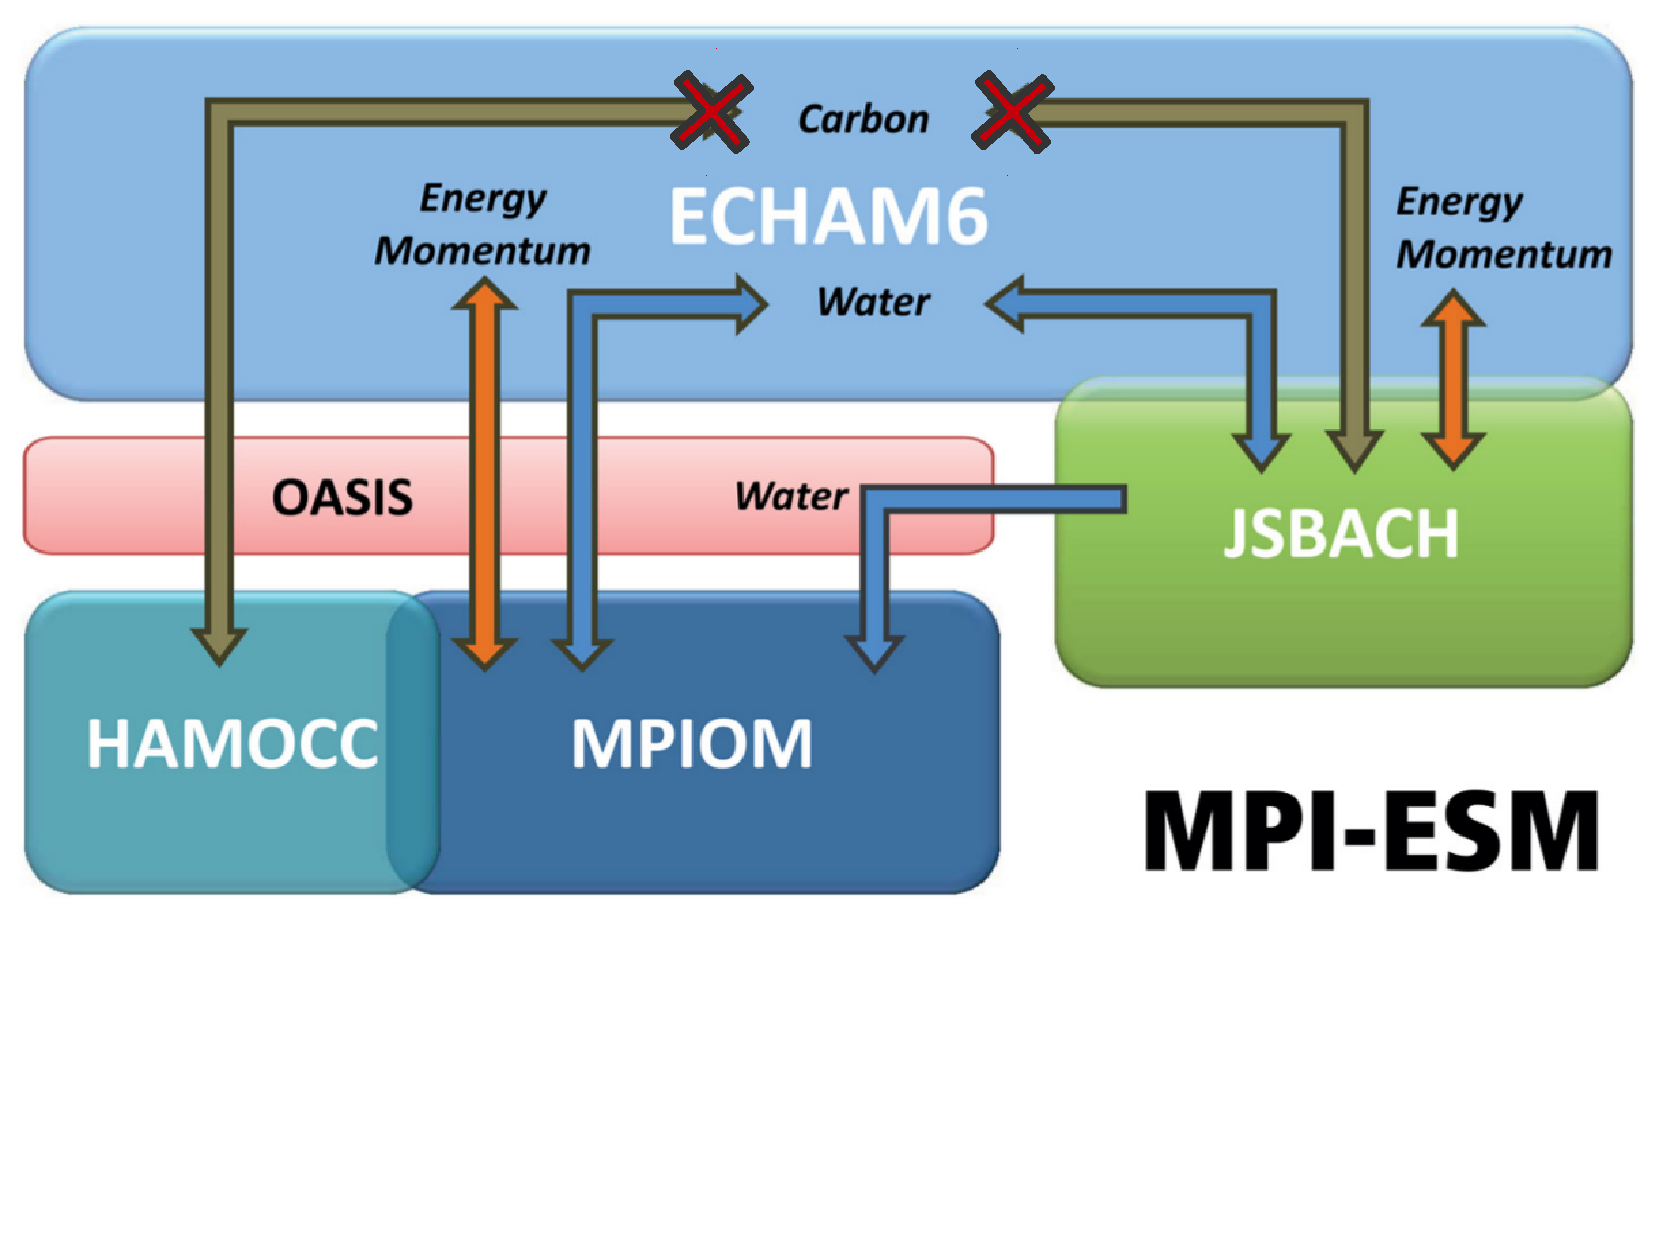
\includegraphics[scale=.42,trim=0cm 6cm 0cm 0cm,clip]{gfx/MPIESM.pdf}
	\caption{Schematic overview on the different components in MPI-Earth-System-Model}
	\label{fig:MPIESM}
\end{figure}

\subsection{HAMOCC}

\section{Large ensemble}
% about ensemble   
An ensemble of 100-member CMIP5 historical simulations and runs under  Representative Concentration Pathway (RCP) 4.5 scenario are integrated for the periods from 1850-2005, and 2006-2100, respectively. Ensemble members differ through starting from different year of the pre-industrial control simulation, so ocean and atmosphere have different initial conditions in each run.  
%ref to CESM ensemble or other ensemble studies?

\section{Fundamental processes of marine biogeochemistry}
no separation but classification, difficult to separate in nature, no single and only cause
\subsection{Physical processes}
\subsection{Biological processes}
\subsection{Chemical processes}

\section{Statistical methods}
which I used
\subsubsection*{Linear Trend}
significance via student t-test

%\subsubsection{•}

%*****************************************
%*****************************************
%*****************************************
%*****************************************
%*****************************************
